% Practice Test 07 — Oklahoma Edition
% Questions: 30 (18 MC + 12 SA)
% Generated by scripts/generate_practice_tests.py

\begin{practiceQuestion}{1-3-q23}{sa}
\begin{questionText}
Two quantities are proportional with $k = 7$. If $y = 56$, what is $x$?
\end{questionText}
\correctAnswer{$x = 8$}
\explanation{$y = kx$ so $56 = 7x$, giving $x = 56 \div 7 = 8$.}
\end{practiceQuestion}

\begin{practiceQuestion}{1-6-q09}{mc}
\begin{questionText}
Which strategy is NOT a proportional reasoning tool?
\end{questionText}
\choiceA{Find the unit rate and multiply}
\choiceB{Set up a proportion and cross-multiply}
\choiceC{Use $y = kx$}
\choiceD{Add a fixed amount to each value}
\correctAnswer{D}
\explanation{Adding a fixed amount is an additive strategy, not proportional. Proportional strategies use multiplication and division.}
\end{practiceQuestion}

\begin{practiceQuestion}{1-7-q29}{gsa}
\begin{questionText}
The scale drawing below shows a garden. Each square represents $1$ cm on the drawing. The scale is $1 : 200$. Find the actual perimeter of the garden in meters.

\begin{center}
\begin{tikzpicture}[scale=0.5]
  \draw[step=1,gray!30,thin] (0,0) grid (10,8);
  \draw[thick,funBlue,fill=green!15] (1,1) rectangle (9,6);
  \draw[<->] (1,0.3) -- (9,0.3) node[midway,below] {$8$ cm};
  \draw[<->] (0.3,1) -- (0.3,6) node[midway,left] {$5$ cm};
  \node at (5,3.5) {Garden};
\end{tikzpicture}
\end{center}
\end{questionText}
\correctAnswer{$52$ m}
\explanation{Model perimeter: $2(8 + 5) = 26$ cm. Actual: $26 \times 200 = 5{,}200$ cm $= 52$ m.}
\end{practiceQuestion}

\begin{practiceQuestion}{2-1-q27}{gmc}
\begin{questionText}
The bar graph shows how many students chose each favorite sport. What percent of the students chose soccer?

\begin{center}
\begin{tikzpicture}[scale=0.55]
  \draw[thick,->] (0,0) -- (0,6.5) node[above]{\small Students};
  \draw[thick,->] (0,0) -- (7,0);
  % Bars
  \fill[funBlue!60] (0.5,0) rectangle (1.5,3);
  \fill[funGreen!60] (2,0) rectangle (3,6);
  \fill[funOrange!60] (3.5,0) rectangle (4.5,4.5);
  \fill[funRed!60] (5,0) rectangle (6,1.5);
  % Labels
  \node[below,font=\small] at (1,0) {Baseball};
  \node[below,font=\small] at (2.5,0) {Soccer};
  \node[below,font=\small] at (4,0) {Basketball};
  \node[below,font=\small] at (5.5,0) {Tennis};
  % Y-axis ticks
  \foreach \y/\lab in {1.5/6,3/12,4.5/18,6/24} {
    \draw (-0.1,\y) -- (0.1,\y) node[left,font=\small,xshift=-2pt] {\lab};
  }
  % Values on bars
  \node[above,font=\small] at (1,3) {$12$};
  \node[above,font=\small] at (2.5,6) {$24$};
  \node[above,font=\small] at (4,4.5) {$18$};
  \node[above,font=\small] at (5.5,1.5) {$6$};
\end{tikzpicture}
\end{center}
\end{questionText}
\choiceA{$24\%$}
\choiceB{$30\%$}
\choiceC{$40\%$}
\choiceD{$50\%$}
\correctAnswer{C}
\explanation{Total students: $12 + 24 + 18 + 6 = 60$. Soccer: $24$. Percent: $24 \div 60 = 0.40 = 40\%$.}
\end{practiceQuestion}

\begin{practiceQuestion}{2-4-q19}{sa}
\begin{questionText}
A store buys a board game for $\$16$ and marks it up $125\%$. What is the selling price?
\end{questionText}
\correctAnswer{$\$36$}
\explanation{$16 \times 2.25 = \$36$.}
\end{practiceQuestion}

\begin{practiceQuestion}{2-7-q21}{sa}
\begin{questionText}
A baker expected to make $80$ cookies from a recipe but made $72$. What is the percent error (rounded to the nearest tenth)?
\end{questionText}
\correctAnswer{$\approx 11.1\%$}
\explanation{$\frac{|80 - 72|}{72} \times 100 = \frac{8}{72} \times 100 \approx 11.1\%$.}
\end{practiceQuestion}

\begin{practiceQuestion}{2-8-q12}{mc}
\begin{questionText}
You owe $\$250$ on a credit card with $20\%$ annual interest. If you pay nothing for $1$ year, how much will you owe?
\end{questionText}
\choiceA{$\$270$}
\choiceB{$\$300$}
\choiceC{$\$275$}
\choiceD{$\$350$}
\correctAnswer{B}
\explanation{Interest $= 250 \times 0.20 = \$50$. Total owed $= 250 + 50 = \$300$.}
\end{practiceQuestion}

\begin{practiceQuestion}{3-1-q04}{mc}
\begin{questionText}
A number plus its opposite always equals which value?
\end{questionText}
\choiceA{$1$}
\choiceB{$-1$}
\choiceC{The number itself}
\choiceD{$0$}
\correctAnswer{D}
\explanation{A number and its opposite are additive inverses. For example, $5 + (-5) = 0$.}
\end{practiceQuestion}

\begin{practiceQuestion}{4-1-q16}{mc}
\begin{questionText}
Evaluate $0.5n + 3.2$ when $n = 6$.
\end{questionText}
\choiceA{$6.2$}
\choiceB{$6.7$}
\choiceC{$9.2$}
\choiceD{$3.7$}
\correctAnswer{A}
\explanation{Substitute: $0.5(6) + 3.2 = 3.0 + 3.2 = 6.2$.}
\end{practiceQuestion}

\begin{practiceQuestion}{4-2-q08}{mc}
\begin{questionText}
Simplify $\frac{1}{3}x + \frac{2}{3}x$.


\begin{center}
\fractionBar{1}{3}
\hspace{1cm}
\fractionBar{2}{3}
\end{center}
\end{questionText}
\choiceA{$\frac{2}{9}x$}
\choiceB{$x$}
\choiceC{$\frac{3}{6}x$}
\choiceD{$\frac{1}{3}x^2$}
\correctAnswer{B}
\explanation{The coefficients are $\frac{1}{3}$ and $\frac{2}{3}$. Add: $\frac{1}{3} + \frac{2}{3} = \frac{3}{3} = 1$. Result: $1x = x$.}
\end{practiceQuestion}

\begin{practiceQuestion}{5-3-q13}{mc}
\begin{questionText}
Solve $-5(x + 1) = -30$.
\end{questionText}
\choiceA{$x = 5$}
\choiceB{$x = -7$}
\choiceC{$x = 7$}
\choiceD{$x = -5$}
\correctAnswer{A}
\explanation{Divide by $-5$: $x + 1 = 6$. Subtract $1$: $x = 5$. Check: $-5(5 + 1) = -5(6) = -30$ \checkmark.}
\end{practiceQuestion}

\begin{practiceQuestion}{5-4-q17}{mc}
\begin{questionText}
Solve $\dfrac{x}{5} + \dfrac{3}{10} = \dfrac{7}{10}$.
\end{questionText}
\choiceA{$x = 4$}
\choiceB{$x = 5$}
\choiceC{$x = 1$}
\choiceD{$x = 2$}
\correctAnswer{D}
\explanation{Multiply every term by $10$: $2x + 3 = 7$. Subtract $3$: $2x = 4$. Divide by $2$: $x = 2$. Check: $\frac{2}{5} + \frac{3}{10} = \frac{4}{10} + \frac{3}{10} = \frac{7}{10}$ \checkmark.}
\end{practiceQuestion}

\begin{practiceQuestion}{5-5-q20}{sa}
\begin{questionText}
Solve $-5n + 10 \leq -15$.
\end{questionText}
\correctAnswer{$n \geq 5$}
\explanation{Subtract $10$: $-5n \leq -25$. Divide by $-5$ and flip: $n \geq 5$.}
\end{practiceQuestion}

\begin{practiceQuestion}{5-6-q26}{gmc}
\begin{questionText}
Which inequality matches the graph below?

\begin{center}
\begin{tikzpicture}[scale=0.7]
  \draw[thick,->] (-5,0) -- (5,0);
  \foreach \x in {-4,...,4} \draw (\x,0.15) -- (\x,-0.15) node[below] {$\x$};
  \draw[thick,funBlue,<-] (-5,0) -- (1,0);
  \fill[funBlue] (1,0) circle (4pt);
\end{tikzpicture}
\end{center}
\end{questionText}
\choiceA{$x \leq 1$}
\choiceB{$x < 1$}
\choiceC{$x \geq 1$}
\choiceD{$x > 1$}
\correctAnswer{A}
\explanation{Closed circle at $1$ with shading to the left means $x \leq 1$.}
\end{practiceQuestion}

\begin{practiceQuestion}{6-2-q29}{gsa}
\begin{questionText}
The rectangle below is drawn at scale $1$ cm $= 8$ m. Redraw it at scale $1$ cm $= 4$ m. What are the new dimensions, and what is the new drawing's area?

\begin{center}
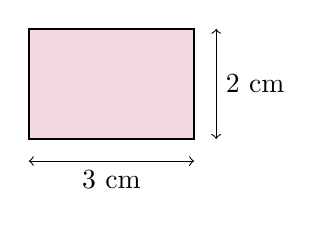
\begin{tikzpicture}[scale=0.7]
  \draw[thick,fill=purple!15] (0,0) rectangle (3,2);
  \draw[<->] (0,-0.4) -- (3,-0.4);
  \node[below] at (1.5,-0.4) {$3$ cm};
  \draw[<->] (3.4,0) -- (3.4,2);
  \node[right] at (3.4,1) {$2$ cm};
\end{tikzpicture}
\end{center}
\end{questionText}
\correctAnswer{$6$ cm by $4$ cm; area $= 24$ cm$^2$}
\explanation{Scale ratio: $\frac{8}{4} = 2$. New dimensions: $3 \times 2 = 6$ cm and $2 \times 2 = 4$ cm. Area: $6 \times 4 = 24$ cm$^2$.}
\end{practiceQuestion}

\begin{practiceQuestion}{6-3-q30}{gsa}
\begin{questionText}
The diagram below shows a triangle attempt with the given side lengths. Explain whether this triangle is possible using the triangle inequality.

\begin{center}
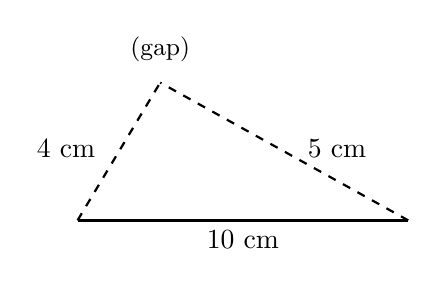
\begin{tikzpicture}[scale=0.7]
  \draw[thick] (0,0) -- (6,0);
  \draw[thick,dashed] (0,0) -- (1.5,2.5);
  \draw[thick,dashed] (6,0) -- (1.5,2.5);
  \node[below] at (3,0) {$10$ cm};
  \node[left] at (0.5,1.3) {$4$ cm};
  \node[right] at (4,1.3) {$5$ cm};
  \node[above] at (1.5,2.7) {\small (gap)};
\end{tikzpicture}
\end{center}
\end{questionText}
\correctAnswer{No, it is not possible}
\explanation{Check: $4 + 5 = 9 < 10$. The two shorter sides cannot connect across the base. The triangle inequality fails, so no triangle can be formed. The dashed lines with the gap illustrate that the sides don't meet.}
\end{practiceQuestion}

\begin{practiceQuestion}{6-4-q24}{sa}
\begin{questionText}
You are given two sides ($5$ cm and $7$ cm) and the included angle ($90°$). Is the resulting triangle unique? What type of triangle is it?
\end{questionText}
\correctAnswer{Yes, unique; it is a right triangle}
\explanation{SAS produces a unique triangle. The included angle of $90°$ makes it a right triangle with legs $5$ cm and $7$ cm.}
\end{practiceQuestion}

\begin{practiceQuestion}{6-5-q19}{sa}
\begin{questionText}
What shape is the cross-section when you cut a sphere through its center?
\end{questionText}
\correctAnswer{A circle (the largest possible circle)}
\explanation{A cut through the center of a sphere produces a great circle — the largest possible circular cross-section, with the same radius as the sphere.}
\end{practiceQuestion}

\begin{practiceQuestion}{6-6-q13}{mc}
\begin{questionText}
Two lines intersect. One angle formed is $130°$. What are the measures of all four angles?
\end{questionText}
\choiceA{$130°$, $130°$, $50°$, $50°$}
\choiceB{$130°$, $50°$, $130°$, $100°$}
\choiceC{$130°$, $130°$, $130°$, $130°$}
\choiceD{$130°$, $60°$, $130°$, $40°$}
\correctAnswer{A}
\explanation{Vertical angles are equal ($130°$ and $130°$). Adjacent angles are supplementary: $180° - 130° = 50°$. The four angles are $130°$, $50°$, $130°$, $50°$.}
\end{practiceQuestion}

\begin{practiceQuestion}{7-4-q16}{mc}
\begin{questionText}
A figure is made of a right triangle with legs $6$ cm and $8$ cm, and a rectangle $8$ cm by $3$ cm. What is the total area?
\end{questionText}
\choiceA{$24$ cm$^2$}
\choiceB{$48$ cm$^2$}
\choiceC{$36$ cm$^2$}
\choiceD{$72$ cm$^2$}
\correctAnswer{B}
\explanation{Triangle: $\frac{1}{2} \times 6 \times 8 = 24$ cm$^2$. Rectangle: $8 \times 3 = 24$ cm$^2$. Total: $24 + 24 = 48$ cm$^2$.}
\end{practiceQuestion}

\begin{practiceQuestion}{7-5-q09}{mc}
\begin{questionText}
A rectangular prism has dimensions $7$ m by $4$ m by $3$ m. What is the area of the largest face?
\end{questionText}
\choiceA{$12$ m$^2$}
\choiceB{$21$ m$^2$}
\choiceC{$28$ m$^2$}
\choiceD{$84$ m$^2$}
\correctAnswer{C}
\explanation{The three pairs of faces have areas $7 \times 4 = 28$, $7 \times 3 = 21$, and $4 \times 3 = 12$ m$^2$. The largest is $28$ m$^2$.}
\end{practiceQuestion}

\begin{practiceQuestion}{7-6-q12}{mc}
\begin{questionText}
A pool is $10$ m long, $5$ m wide, and $2$ m deep. How many cubic meters of water does it hold when full?
\end{questionText}
\choiceA{$17$ m$^3$}
\choiceB{$50$ m$^3$}
\choiceC{$100$ m$^3$}
\choiceD{$200$ m$^3$}
\correctAnswer{C}
\explanation{$V = 10 \times 5 \times 2 = 100$ m$^3$.}
\end{practiceQuestion}

\begin{practiceQuestion}{8-1-q08}{mc}
\begin{questionText}
A sample of $40$ out of $2{,}000$ voters is surveyed. What fraction of the population is in the sample?
\end{questionText}
\choiceA{$\frac{1}{50}$}
\choiceB{$\frac{1}{40}$}
\choiceC{$\frac{1}{20}$}
\choiceD{$\frac{1}{500}$}
\correctAnswer{A}
\explanation{$\frac{40}{2{,}000} = \frac{1}{50}$.}
\end{practiceQuestion}

\begin{practiceQuestion}{8-3-q26}{gmc}
\begin{questionText}
The box plots below compare test scores for Class A and Class B.

\begin{center}
\begin{tikzpicture}[scale=0.1]
  \draw[thick,->] (49,0) -- (101,0);
  \foreach \x in {50,55,...,100} {
    \draw (\x,0.5) -- (\x,-0.5);
    \node[below,font=\small] at (\x,-0.5) {$\x$};
  }
  % Class A: min=60, Q1=70, med=78, Q3=85, max=95
  \draw[thick] (60,6) -- (95,6);
  \draw[thick,fill=funBlue!30] (70,4) rectangle (85,8);
  \draw[very thick,funBlue] (78,4) -- (78,8);
  \draw[thick] (60,4) -- (60,8);
  \draw[thick] (95,4) -- (95,8);
  \node[right,font=\small] at (96,6) {Class A};
  % Class B: min=50, Q1=58, med=65, Q3=72, max=80
  \draw[thick] (50,14) -- (80,14);
  \draw[thick,fill=funGreen!30] (58,12) rectangle (72,16);
  \draw[very thick,funGreen] (65,12) -- (65,16);
  \draw[thick] (50,12) -- (50,16);
  \draw[thick] (80,12) -- (80,16);
  \node[right,font=\small] at (81,14) {Class B};
\end{tikzpicture}
\end{center}

Which statement is best supported by the box plots?
\end{questionText}
\choiceA{Class B scored higher than Class A}
\choiceB{Class A has a higher median and a larger IQR}
\choiceC{Class A has a higher median and both classes have the same IQR}
\choiceD{Class A and Class B overlap, but Class A's median is higher}
\correctAnswer{D}
\explanation{Class A median $= 78$, Class B median $= 65$. Class A's range ($60$--$95$) overlaps with Class B's range ($50$--$80$), but Class A is higher overall.}
\end{practiceQuestion}

\begin{practiceQuestion}{8-4-q13}{mc}
\begin{questionText}
Store A daily sales: mean $\$500$, MAD $\$40$. Store B daily sales: mean $\$620$, MAD $\$40$. The difference in means in MADs is:
\end{questionText}
\choiceA{$1.5$ MADs}
\choiceB{$3$ MADs}
\choiceC{$40$ MADs}
\choiceD{$120$ MADs}
\correctAnswer{B}
\explanation{Difference $= \$620 - \$500 = \$120$. In MADs: $\frac{120}{40} = 3$ MADs.}
\end{practiceQuestion}

\begin{practiceQuestion}{8-5-q15}{mc}
\begin{questionText}
What is the mean of the data shown?

\begin{center}
\begin{tabular}{r|l}
\textbf{Stem} & \textbf{Leaf} \\
\hline
$1$ & $0\;\;5$ \\
$2$ & $0\;\;5$ \\
$3$ & $0$
\end{tabular}
\end{center}
\end{questionText}
\choiceA{$15$}
\choiceB{$18$}
\choiceC{$20$}
\choiceD{$25$}
\correctAnswer{C}
\explanation{Data: $10, 15, 20, 25, 30$. Mean $= \frac{10+15+20+25+30}{5} = \frac{100}{5} = 20$.}
\end{practiceQuestion}

\begin{practiceQuestion}{8-7-q19}{sa}
\begin{questionText}
A frequency table shows: Soccer $15$, Basketball $20$, Tennis $10$, Swimming $5$. What is the total and what percent play basketball?
\end{questionText}
\correctAnswer{Total $= 50$; Basketball $= 40\%$}
\explanation{$15+20+10+5 = 50$. Basketball: $\frac{20}{50} = 40\%$.}
\end{practiceQuestion}

\begin{practiceQuestion}{9-4-q30}{gsa}
\begin{questionText}
The table below shows a probability model for a game spinner. One probability is missing. Find the missing probability for outcome D.

\begin{center}
\begin{tabular}{|c|c|}
\hline
\textbf{Outcome} & \textbf{Probability} \\
\hline
A & $0.30$ \\
\hline
B & $0.25$ \\
\hline
C & $0.15$ \\
\hline
D & ? \\
\hline
\end{tabular}
\end{center}
\end{questionText}
\correctAnswer{$0.30$}
\explanation{$P(D) = 1 - (0.30 + 0.25 + 0.15) = 1 - 0.70 = 0.30$.}
\end{practiceQuestion}

\begin{practiceQuestion}{9-6-q06}{mc}
\begin{questionText}
Two dice are rolled. What is the probability that both dice show the same number (doubles)?
\end{questionText}
\choiceA{$\frac{1}{36}$}
\choiceB{$\frac{1}{12}$}
\choiceC{$\frac{1}{6}$}
\choiceD{$\frac{1}{3}$}
\correctAnswer{C}
\explanation{Doubles: $(1,1), (2,2), (3,3), (4,4), (5,5), (6,6)$ — that is $6$ out of $36$. $P = \frac{6}{36} = \frac{1}{6}$.}
\end{practiceQuestion}

\begin{practiceQuestion}{9-7-q25}{sa}
\begin{questionText}
A student runs $200$ simulation trials for an event with theoretical probability $\frac{1}{4}$. They observe the event $54$ times. What is the experimental probability? Is it close to the theoretical value?
\end{questionText}
\correctAnswer{$0.27$; yes, it is close to $0.25$}
\explanation{$P = \frac{54}{200} = 0.27$. Theoretical $= 0.25$. The difference of $0.02$ is small, especially with $200$ trials.}
\end{practiceQuestion}
